\chapter{Results and Discussion}

\section{Termination Step of P3HT Synthesis}

The first problem tackled in this project was to develop an inline procedure for properly terminating the polymerisation prior to passing it through the separation and analysis stages of the flow reactor. Small amounts of unreacted Grignard monomer in the reaction mixture can cause the polymerisation to continue once the droplets have left the oil bath, causing the polymer chain length to increase during the analysis step. This leads to unreliable measurements, and at high molecular weights can cause precipitation of the product polymer inside the GPC column, causing blockages (which require multiple cleaning washes to remove) or even breaking the elution chamber.

Initially, the introduction of a wash was considered. The wash solvent ideally would be able to extract the unreacted Grignard species from the THF phase, and be immiscible with THF itself. However, it was crucial not to introduce a wash that caused precipitation of the polymer out of the THF phase. The use of ionic liquids (ILs) was investigated, with a paper published by O. Kuzmina et. al. and the thesis of P. J. Corbytt showing the ability of the ionic liquid 1-butyl-3-methylimidazolium acetate ([bmim][OAc]) to remove group 1 and transition metal salts from solution, with the aim to remove any leftover unreacted Grignard reagent from solution. However, due to the amount of IL needed to wash the reaction mixture over an extended period, the cost and volume of waste produced would be too high for an efficient continuous process. Therefore, alternative methods were investigated.

The introduction of a solution of a non-selective GRIM catalyst could potentially be used to react together any unused monomers, including the minority isomer that leads to undesirable couplings. The resultant formation of dithiophene in the reaction mixture was not expected to interfere with the analysis due to its very low molecular weight.  

To form solely dithiophene molecules instead of longer chain oligomers, the catalyst should be added in excess compared to the number of unreacted monomers left in solution. The concentration of catalyst needed to obtain a 1:1 ratio of monomer unit to active non-selective catalyst centre for a completely unreacted monomer solution was calculated assuming the same flow rate of the non-selective catalyst solution as the Ni(dppp)Br2 solution, shown in Figure 15. 



\subsection{Production of Non-Selective Catalyst Solution}

The active non-selective catalyst must be formed in solution due to its low solubility in THF. Different target concentrations of Ni(TPP)2Br2 were attempted to be made by adding different quantities of Ni(dme)Br2 and TPP to THF under inert conditions. A summary of the results can be seen in Table 1 below.

\begin{table}[]
	\begin{tabular}{llll}
		Catalyst Loading /mol \% & Ni(dme)Br2 /g & PPh3 /g & Notes         \\
		50                       & 0.386         & 0.918   & Not dissolved \\
		15                       &               &         & Dissolved    
	\end{tabular}
\end{table}

A molar ratio of at least 3:1 TPP to Ni(dme)Br2 was used to shift the ligand exchange equilibrium towards the bis-triphosphino complex. The X M solution was selected for use as it dissolved completely, and contained sufficient Ni(TPP)2Br2 catalyst to fully quench all active species in the monomer solution.

\subsection{Testing of Reaction Termination}

To test whether the Ni(TPP)2Br2 solution would indeed terminate the GRIM reaction, a batch synthesis of P3HT was performed as outlined in the experimental section. At regular time intervals aliquots of the reaction mixture were withdrawn from the reaction flask with a syringe, and quenched in acidified methanol to cause precipitation of the product P3HT. The result can be seen in Figure 14 below.

\includegraphics{AliquotQuick}

Initially the molecular weight of the P3HT was observed to increase at an approximately constant rate of X/min. However, after approximately six minutes the reaction slowed considerably, consistent with the quasi-living chain growth mechanism, described in Chapter 1. The reaction was then repeated with a more dilute reaction, by halving the concentration of the reagents as so to increase the duration of the “living” growth phase with a view to allowing sufficient time for Ni(TPP)2Br2 addition in later experiments. The results are shown in Figure 15.

\includegraphics{AliquotLong}

Under the diluted conditions used, the “living” growth phase lasted approximately ten minutes, sufficiently long for Ni(TPP)2Br2 addition. The reaction was then repeated with the same conditions, but a solution of Ni(TPP)2Br2 was injected into the flask at the five-minute mark. The result can be seen in Figure 16.

\includegraphics{AliquotTermination}

Upon injection of the catalyst solution, the molecular weight of P3HT plateaued at just over 32 kDa, and did not increase further over a period of ninety minutes, indicating that the reaction had successfully been terminated. The high value of Mn obtained on the 5-minute mark occurred because the withdrawn aliquot was held in the syringe longer whilst the catalyst solution was injected into the reaction flask, leaving the polymer to grow for a longer time before being quenched.

\subsection{Introduction of Termination Step in Flow}

Once the ability to terminate the polymerisation reaction was shown, it was implemented into the droplet flow reactor. The previous reactor setup was modified to include an additional flow mixer, as shown in Figure 17.

\includegraphics{HerringtonReactor}
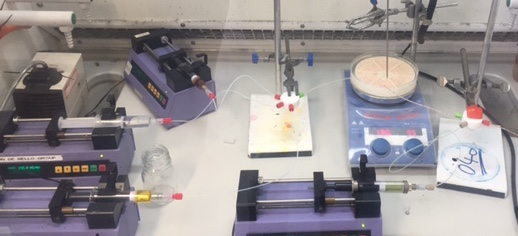
\includegraphics{JackReactor}

To determine whether the termination would supress unwanted coupling and precipitation inside the GPC column, a droplet flow synthesis was run over an extended time, and monitored periodically via the GPC instrument to show long term stability. The transmission response for each successive GPC trace can be seen in Figure 18.

\includegraphics{2hours}

Each GPC analysis takes 15 minutes to run to completion, and the reaction was run for 75 minutes, allowing for five successive analyses to be completed. All the traces show 2 distinct peaks at X and Y, as opposed to the desired single peak, indicative of polymer samples of two separate lengths, which may have arisen from termination step causing the synthesis of short chain oligomers from the remaining monomer in solution. The signals vary in intensity, which indicates that the different samples injected had different concentrations of P3HT. The yellow trace shows additional noise following the expected signal. This occurred due to the improper separation of the two-phase droplet flow, resulting in the inclusion of some Galden in the GPC sample. This issue required a more in-depth look at the liquid-liquid separator and monitoring of the separation quality, as so to prevent future contamination of the GPC column.

\section{Liquid-Liquid Separator Design}

